\documentclass[aspectratio=169,12pt]{beamer}
\usepackage[utf8]{inputenc}
\usepackage{graphicx}
\usepackage{tikz}
\usepackage{array}
\usepackage{booktabs}
\usepackage{colortbl}
\usepackage{xcolor}

\usetikzlibrary{shapes,arrows,positioning,shadows,calc}

% Theme
\usetheme{Madrid}
\usecolortheme{default}

% Colors
\definecolor{darkblue}{RGB}{0,51,102}
\definecolor{lightblue}{RGB}{102,153,204}
\definecolor{orange}{RGB}{255,102,0}
\definecolor{lightgray}{RGB}{240,240,240}

\setbeamercolor{structure}{fg=darkblue}
\setbeamercolor{frametitle}{bg=darkblue,fg=white}
\setbeamercolor{title}{bg=darkblue,fg=white}

% Title page
\title[Dal Modello E-R allo Schema Logico]{Dal Modello Entità-Relazione allo Schema Logico}
\subtitle{Progettazione di Database}
\author{Prof. Fedeli Massimo}
\institute{ITS 4.0 - Tutti i diritti riservati}
\date{A.S. 2025/26}

\begin{document}

% Slide 1 - Title
\begin{frame}
\titlepage
\end{frame}

% Slide 2 - Table of Contents
\begin{frame}{Contenuti}
\tableofcontents
\end{frame}

\section{Introduzione alla Progettazione Logica}

% Slide 3
\begin{frame}{Progettazione Logica: Obiettivo}
\begin{block}{Obiettivo}
Costruire uno \textbf{schema logico} in grado di descrivere, in maniera corretta ed efficiente, tutte le informazioni contenute nello schema Entità-Relazione prodotto nella fase di progettazione concettuale.
\end{block}

\vspace{0.5cm}

\begin{alertblock}{Importante}
Non è una semplice traduzione da un modello a un altro!
\end{alertblock}
\end{frame}

% Slide 4
\begin{frame}{Progettazione Logica: Ristrutturazione}
Prima di passare allo schema logico, lo schema E-R va \textbf{ristrutturato} per:

\begin{enumerate}
\item \textcolor{orange}{\textbf{Semplificare}} la traduzione
\item \textcolor{orange}{\textbf{Ottimizzare}} il progetto
\end{enumerate}

\vspace{0.5cm}

\begin{block}{Ricorda}
La progettazione concettuale ha come obiettivo la rappresentazione accurata e naturale dei dati dal punto di vista del \textit{significato}.
\end{block}
\end{frame}

% Slide 5
\begin{frame}{Progettazione Logica: Base per l'Applicazione}
\begin{columns}
\begin{column}{0.6\textwidth}
La progettazione logica costituisce la \textcolor{orange}{\textbf{base per l'effettiva realizzazione dell'applicazione}} e deve tener conto, per quanto possibile, delle sue \textcolor{darkblue}{\textbf{prestazioni}}.

\vspace{0.5cm}

Questa necessità può portare a una \textbf{ristrutturazione} dello schema concettuale che renda più efficiente l'esecuzione delle operazioni previste.
\end{column}
\begin{column}{0.4\textwidth}
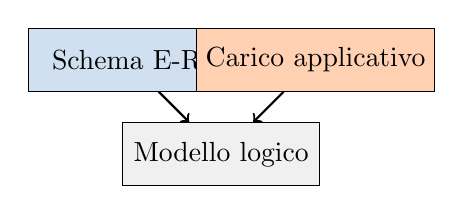
\begin{tikzpicture}[scale=0.8]
\node[rectangle, draw, fill=lightblue!30, minimum width=2.5cm, minimum height=0.8cm] (er) at (0,3) {Schema E-R};
\node[rectangle, draw, fill=orange!30, minimum width=2.5cm, minimum height=0.8cm] (app) at (3,3) {Carico applicativo};
\node[rectangle, draw, fill=lightgray, minimum width=2.5cm, minimum height=0.8cm] (log) at (1.5,1.5) {Modello logico};

\draw[->, thick] (er) -- (log);
\draw[->, thick] (app) -- (log);
\end{tikzpicture}
\end{column}
\end{columns}
\end{frame}

% Slide 6
\begin{frame}{Le Due Fasi}
È necessario prevedere:
\begin{enumerate}
\item Un'attività di \textcolor{orange}{\textbf{riorganizzazione}}
\item Un'attività di \textcolor{darkblue}{\textbf{traduzione}}
\end{enumerate}

\vspace{0.5cm}

La progettazione logica si articola quindi in \textbf{due fasi}:
\begin{itemize}
\item \textbf{Ristrutturazione} dello schema Entità-Relazione
\item \textbf{Traduzione} verso il modello logico
\end{itemize}
\end{frame}

% Slide 7
\begin{frame}{Processo di Progettazione}
\begin{center}
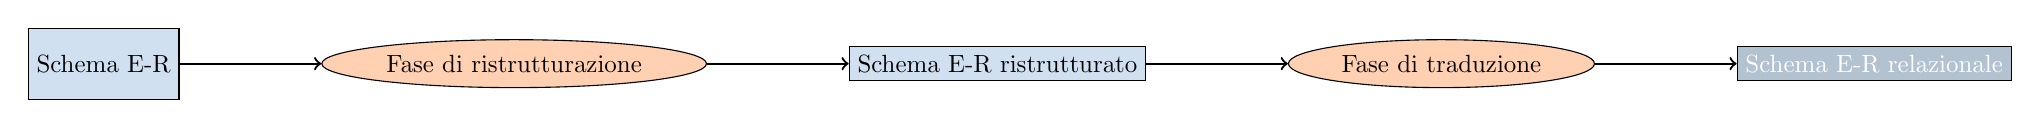
\begin{tikzpicture}[node distance=2cm, scale=0.9, transform shape]
\node[rectangle, draw, fill=lightblue!30, minimum width=2cm, minimum height=1cm] (er1) {Schema E-R};
\node[ellipse, draw, fill=orange!30, right=of er1] (rist) {Fase di ristrutturazione};
\node[rectangle, draw, fill=lightblue!30, right=of rist, minimum width=2.5cm] (er2) {Schema E-R ristrutturato};
\node[ellipse, draw, fill=orange!30, right=of er2] (trad) {Fase di traduzione};
\node[rectangle, draw, fill=darkblue!30, text=white, right=of trad, minimum width=2.5cm] (rel) {Schema E-R relazionale};

\draw[->, thick] (er1) -- (rist);
\draw[->, thick] (rist) -- (er2);
\draw[->, thick] (er2) -- (trad);
\draw[->, thick] (trad) -- (rel);
\end{tikzpicture}
\end{center}
\end{frame}

% Slide 8
\begin{frame}{Output della Progettazione Logica}
\begin{columns}
\begin{column}{0.5\textwidth}
Costituiscono i prodotti finali:
\begin{itemize}
\item \textbf{Lo schema logico finale}
\item \textbf{I vincoli di integrità} definiti su di esso
\item \textbf{La relativa documentazione}
\end{itemize}
\end{column}
\begin{column}{0.5\textwidth}
\begin{block}{Esempio}
\small
\texttt{Musei(CodiceMuseo, Denominazione, Città, Indirizzo, NumeroOpere)}
\end{block}
\end{column}
\end{columns}
\end{frame}

% Slide 9
\begin{frame}{Il Modello Logico}
Il \textbf{modello logico} del database (o schema logico) è lo strumento che viene utilizzato come \textit{input} per la \textcolor{orange}{\textbf{progettazione fisica}} dei database.

\vspace{0.5cm}

Deve quindi avere il \textcolor{darkblue}{\textbf{massimo livello di dettaglio e precisione possibile}}.

\vspace{0.5cm}

\begin{alertblock}{Funzioni del Modello Logico}
Dota i dati di una struttura utile per \textbf{realizzare}, \textbf{semplificare} e \textbf{ottimizzare} le operazioni di archiviazione, interrogazione e manipolazione dei dati.
\end{alertblock}
\end{frame}

% Slide 10
\begin{frame}{Modello Logico: Contenuti}
Deve contenere tutte le informazioni necessarie per \textbf{definire fisicamente le tabelle}, riportando la \textcolor{orange}{\textbf{descrizione puntuale e completa}} del significato di ogni dato che viene memorizzato.

\vspace{0.5cm}

\begin{block}{Esempio Schema Relazionale}
\texttt{alunni (matricola(pk), cognome, nome, ..., scuola(fk))}
\end{block}

\vspace{0.3cm}

Questo può essere considerato come \textit{schema logico}, ma è sempre preferibile realizzare un \textcolor{darkblue}{\textbf{modello logico preciso}} (o completo) per rendere più semplice la progettazione fisica.
\end{frame}

\section{Modello Logico Preciso}

% Slide 11
\begin{frame}{Componenti del Modello Logico Preciso}
Un modello logico preciso comprende:
\begin{enumerate}
\item Per ogni \textbf{entità}, l'elenco completo degli attributi
\item Per ogni \textbf{entità}, l'indicazione esplicita della chiave primaria e di eventuali chiavi alternative
\item Per ogni \textbf{entità}, l'indicazione esplicita di eventuali chiavi esterne
\item Per ogni \textbf{attributo}, l'indicazione esplicita di opzionalità o obbligatorietà
\end{enumerate}
\end{frame}

% Slide 12
\begin{frame}{Componenti del Modello Logico Preciso (2)}
\begin{enumerate}
\setcounter{enumi}{4}
\item Per ogni \textbf{attributo}, l'indicazione esplicita del tipo di dati (\textit{data type}), che ne specifichi il formato e la lunghezza, con la segnalazione dei valori ammessi
\item Per ogni \textbf{relazione}, l'indicazione della molteplicità minima e massima in entrambe le direzioni
\item Per ogni \textbf{relazione}, l'indicazione delle regole di integrità referenziale applicabili
\end{enumerate}
\end{frame}

% Slide 13
\begin{frame}{Esempio: Modello Logico Preciso}
\begin{center}
\small
\begin{tabular}{|l|l|l|l|l|}
\hline
\rowcolor{lightblue!50}
\textbf{Attributo/campo} & \textbf{Tipo} & \textbf{Dimensione} & \textbf{Valori} & \textbf{Note} \\
\hline
Matricola & Numerico & 8 & Autoincrement & pk \\
\hline
Cognome & Stringa & 40 & Not null & \\
\hline
Nome & Stringa & 30 & Not null & \\
\hline
... & & & & \\
\hline
Scuola & Numerico & 12 & Codifica del MIUR & fk \\
\hline
\end{tabular}
\end{center}

\vspace{0.3cm}
Durante la progettazione logica si definiscono inoltre gli \textcolor{orange}{\textbf{schemi esterni (viste)}} per le specifiche applicazioni.
\end{frame}

\section{Ristrutturazione dello Schema E-R}

% Slide 14
\begin{frame}{Ristrutturazione: Panoramica}
Una volta che lo schema E-R è stato completamente definito, si procede al suo \textbf{affinamento} (ristrutturazione) attraverso:

\vspace{0.5cm}

\begin{block}{Regola Base}
\textbf{Eliminazione dei costrutti non rappresentabili} applicando delle regole base di modellizzazione
\end{block}
\end{frame}

% Slide 15
\begin{frame}{Eliminazione Costrutti: Entità Scollegate}
\begin{columns}
\begin{column}{0.6\textwidth}
Le \textbf{entità non possono} essere modellate se sono \textcolor{red}{\textbf{scollegate}} da altre entità.

\vspace{0.5cm}

\begin{block}{Eccezione}
Un database formato da una \textit{singola tabella} (esempio: carrello elettronico nei siti di commercio elettronico)
\end{block}
\end{column}
\begin{column}{0.4\textwidth}
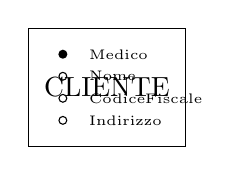
\begin{tikzpicture}[scale=0.7]
\node[rectangle, draw, minimum width=2cm, minimum height=1.5cm] (cliente) at (0,0) {CLIENTE};
\node[circle, draw, fill=black, scale=0.3] at (-0.8,0.6) {};
\node[circle, draw, scale=0.3] at (-0.8,0.2) {};
\node[circle, draw, scale=0.3] at (-0.8,-0.2) {};
\node[circle, draw, scale=0.3] at (-0.8,-0.6) {};
\node[right] at (-0.5,0.6) {\tiny Medico};
\node[right] at (-0.5,0.2) {\tiny Nome};
\node[right] at (-0.5,-0.2) {\tiny CodiceFiscale};
\node[right] at (-0.5,-0.6) {\tiny Indirizzo};
\end{tikzpicture}
\end{column}
\end{columns}
\end{frame}

% Slide 16
\begin{frame}{Eliminazione Attributi Composti}
Nel caso fosse presente un \textbf{attributo composto} si può procedere in due modi alternativi:

\begin{enumerate}
\item \textcolor{darkblue}{\textbf{Considerare}} tutti i sottoattributi come attributi
\item \textcolor{orange}{\textbf{Eliminare}} i sottoattributi e considerare l'attributo composto come un attributo semplice
\end{enumerate}

\vspace{0.5cm}

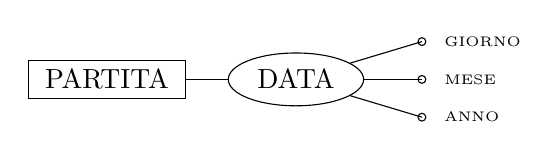
\begin{tikzpicture}[scale=0.8]
\node[rectangle, draw, minimum width=2cm] (partita) at (0,0) {PARTITA};
\node[ellipse, draw] (data) at (3,0) {DATA};
\node[circle, draw, scale=0.3] at (5,0.6) {};
\node[circle, draw, scale=0.3] at (5,0) {};
\node[circle, draw, scale=0.3] at (5,-0.6) {};
\node[right] at (5.2,0.6) {\tiny GIORNO};
\node[right] at (5.2,0) {\tiny MESE};
\node[right] at (5.2,-0.6) {\tiny ANNO};

\draw (partita) -- (data);
\draw (data) -- (5,0.6);
\draw (data) -- (5,0);
\draw (data) -- (5,-0.6);
\end{tikzpicture}
\end{frame}

% Slide 17
\begin{frame}{Attributi Composti: Soluzione A}
\textbf{Soluzione A: scomposizione}

\vspace{0.3cm}

Nell'entità \texttt{studente} è presente come attributo composto il \texttt{nr\_telefono}.

\begin{center}
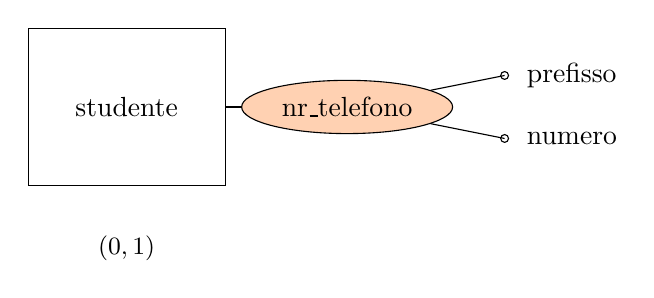
\begin{tikzpicture}[scale=0.8]
\node[rectangle, draw, minimum width=2.5cm, minimum height=2cm] (studente) at (0,0) {studente};
\node[ellipse, draw, fill=orange!30] (tel) at (3.5,0) {nr\_telefono};
\node[circle, draw, scale=0.3] at (6,0.5) {};
\node[circle, draw, scale=0.3] at (6,-0.5) {};
\node[right] at (6.2,0.5) {prefisso};
\node[right] at (6.2,-0.5) {numero};

\draw (studente) -- (tel);
\draw (tel) -- (6,0.5);
\draw (tel) -- (6,-0.5);

\node[below=0.5cm of studente] {\small $(0,1)$};
\end{tikzpicture}
\end{center}

Si scompone in: \texttt{tel\_prefisso} e \texttt{tel\_numero}
\end{frame}

% Slide 18
\begin{frame}{Attributi Composti: Soluzione B}
\textbf{Soluzione B: non considerazione}

\vspace{0.3cm}

\begin{center}
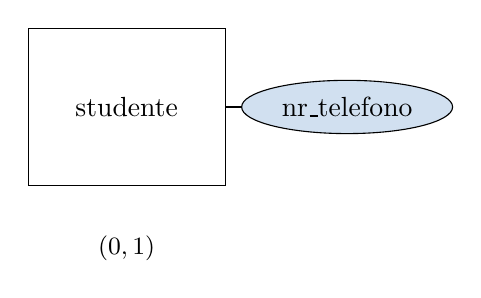
\begin{tikzpicture}[scale=0.8]
\node[rectangle, draw, minimum width=2.5cm, minimum height=2cm] (studente) at (0,0) {studente};
\node[ellipse, draw, fill=lightblue!30] (tel) at (3.5,0) {nr\_telefono};

\draw (studente) -- (tel);

\node[below=0.5cm of studente] {\small $(0,1)$};
\end{tikzpicture}
\end{center}

Si mantiene come unico attributo: \texttt{nr\_telefono}
\end{frame}

% Slide 19
\begin{frame}{Eliminazione Attributi Multivalore}
Gli eventuali \textbf{attributi multivalore} presenti devono essere \textcolor{orange}{\textbf{"promossi" a entità}}.

\vspace{0.5cm}

Si crea una \textit{nuova entità} che contiene i valori dell'attributo e la si collega all'entità che possedeva l'attributo mediante una nuova relazione \textbf{uno-a-molti} o \textbf{molti-a-molti}, a seconda dei casi.
\end{frame}

% Slide 20
\begin{frame}{Attributi Multivalore: Esempio 1}
\textbf{Esempio:} Uno studente può parlare più di una lingua.

\vspace{0.3cm}

\begin{center}
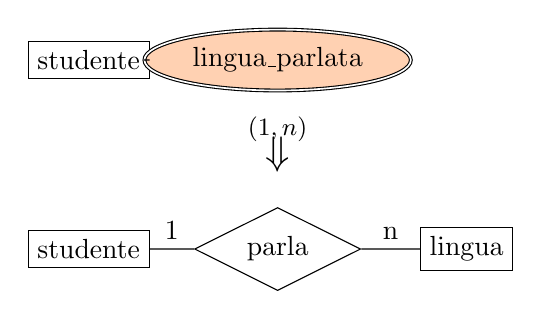
\begin{tikzpicture}[scale=0.8]
% Prima
\node[rectangle, draw] (stud1) at (0,2) {studente};
\node[ellipse, draw, fill=orange!30, double] (lingua1) at (3,2) {lingua\_parlata};
\draw (stud1) -- (lingua1);
\node[below=0.2cm of lingua1] {\small $(1,n)$};

% Dopo
\node[rectangle, draw] (stud2) at (0,-1) {studente};
\node[diamond, draw, aspect=2] (parla) at (3,-1) {parla};
\node[rectangle, draw] (lingua2) at (6,-1) {lingua};

\draw (stud2) -- node[above] {1} (parla);
\draw (parla) -- node[above] {n} (lingua2);

\node at (3,0.5) {\Large $\Downarrow$};
\end{tikzpicture}
\end{center}
\end{frame}

% Slide 21
\begin{frame}{Attributi Multivalore: Esempio 2}
\textbf{Esempio:} Un'azienda può possedere più numeri di telefono.

\vspace{0.3cm}

\begin{center}
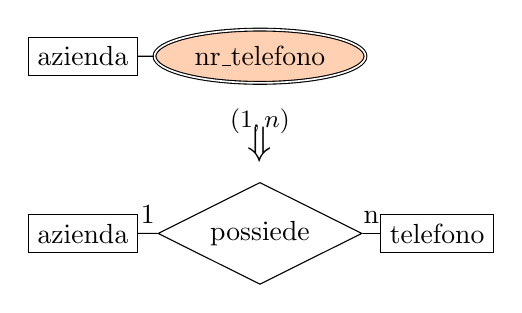
\begin{tikzpicture}[scale=0.75]
% Prima
\node[rectangle, draw] (az1) at (0,2) {azienda};
\node[ellipse, draw, fill=orange!30, double] (tel1) at (3,2) {nr\_telefono};
\draw (az1) -- (tel1);
\node[below=0.2cm of tel1] {\small $(1,n)$};

% Dopo
\node[rectangle, draw] (az2) at (0,-1) {azienda};
\node[diamond, draw, aspect=2] (poss) at (3,-1) {possiede};
\node[rectangle, draw] (tel2) at (6,-1) {telefono};

\draw (az2) -- node[above] {1} (poss);
\draw (poss) -- node[above] {n} (tel2);

\node at (3,0.5) {\Large $\Downarrow$};
\end{tikzpicture}
\end{center}
\end{frame}

% Slide 22
\begin{frame}{Attributi Multivalore: Esempio 3}
\begin{center}
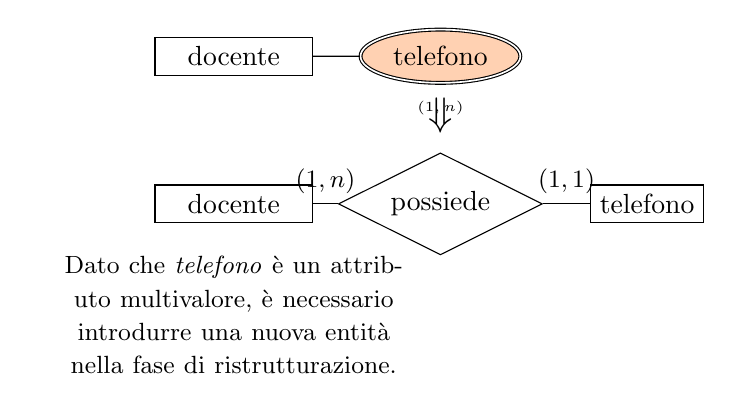
\begin{tikzpicture}[scale=0.75]
% Prima
\node[rectangle, draw, minimum width=2cm] (doc1) at (0,2.5) {docente};
\node[ellipse, draw, fill=orange!30, double] (tel1) at (3.5,2.5) {telefono};
\draw (doc1) -- (tel1);
\node[below=0.1cm of tel1] {\tiny $(1,n)$};

% Dopo
\node[rectangle, draw, minimum width=2cm] (doc2) at (0,0) {docente};
\node[diamond, draw, aspect=2] (poss) at (3.5,0) {possiede};
\node[rectangle, draw] (tel2) at (7,0) {telefono};

\draw (doc2) -- node[above] {\small $(1,n)$} (poss);
\draw (poss) -- node[above] {\small $(1,1)$} (tel2);

\node at (3.5,1.5) {\Large $\Downarrow$};

\node[below=0.3cm of doc2, text width=5cm, align=center] {\small Dato che \textit{telefono} è un attributo multivalore, è necessario introdurre una nuova entità nella fase di ristrutturazione.};
\end{tikzpicture}
\end{center}
\end{frame}

\section{Eliminazione Gerarchie}

% Slide 23
\begin{frame}{Eliminazione Gerarchie e Specializzazioni}
La \textbf{gerarchia di generalizzazione} deve essere trasformata in una unica entità in quanto non è supportata dal modello relazionale.

\vspace{0.5cm}

È possibile ristrutturare il diagramma in due modi differenti:
\begin{enumerate}
\item \textcolor{darkblue}{\textbf{Eliminazione dei figli}} (collasso dei figli), aggiungendo uno o più attributi nell'entità padre
\item \textcolor{orange}{\textbf{Eliminazione del padre}} (esplosione dei figli): completando ciascun figlio con gli attributi del padre
\end{enumerate}
\end{frame}

% Slide 24
\begin{frame}{Gerarchia: Esempio}
\begin{center}
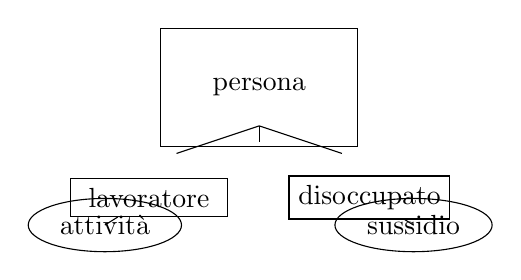
\begin{tikzpicture}[scale=0.7]
\node[rectangle, draw, minimum width=2.5cm, minimum height=1.5cm] (persona) at (3,3) {persona};

\draw (1.5,1.8) -- (3,2.3);
\draw (4.5,1.8) -- (3,2.3);
\draw (3,2.3) -- (3,2);
\node at (3,2) {$\blacktriangle$};

\node[rectangle, draw, minimum width=2cm] (lav) at (1,1) {lavoratore};
\node[rectangle, draw, minimum width=2cm] (dis) at (5,1) {disoccupato};

\node[ellipse, draw] at (5.8,0.5) {sussidio};
\node[ellipse, draw] at (0.2,0.5) {attività};

\draw (lav) -- (0.2,0.5);
\draw (dis) -- (5.8,0.5);
\end{tikzpicture}
\end{center}

Le entità \textit{lavoratore} e \textit{disoccupato} sono figlie dell'entità \textit{persona}.
\end{frame}

% Slide 25
\begin{frame}{Soluzione A: Collasso dei Figli}
\textbf{Caso A:} Una sola entità nella quale sono stati aggiunti gli attributi che rimarranno vuoti a seconda del caso della singola istanza.

\begin{center}
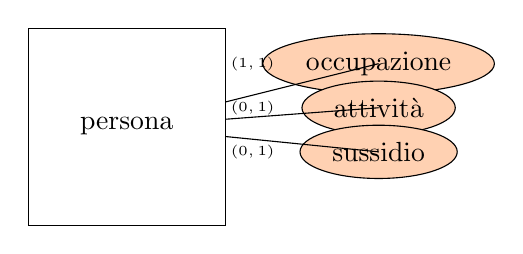
\begin{tikzpicture}[scale=0.8]
\node[rectangle, draw, minimum width=2.5cm, minimum height=2.5cm] (persona) at (0,0) {persona};
\node[ellipse, draw, fill=orange!30] at (4,1) {occupazione};
\node[ellipse, draw, fill=orange!30] at (4,0.3) {attività};
\node[ellipse, draw, fill=orange!30] at (4,-0.4) {sussidio};

\node[right] at (1.5,1) {\tiny $(1,1)$};
\node[right] at (1.5,0.3) {\tiny $(0,1)$};
\node[right] at (1.5,-0.4) {\tiny $(0,1)$};

\draw (persona) -- (4,1);
\draw (persona) -- (4,0.3);
\draw (persona) -- (4,-0.4);
\end{tikzpicture}
\end{center}
\end{frame}

% Slide 26
\begin{frame}{Soluzione B: Esplosione dei Figli}
\textbf{Caso B:} Due entità distinte.

\begin{center}
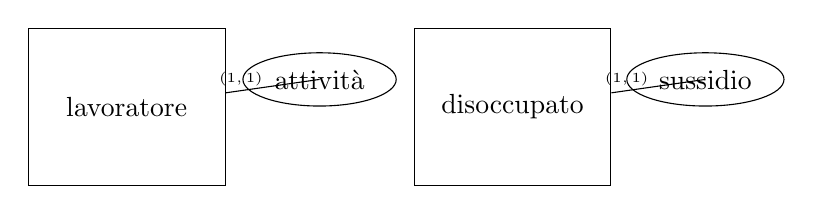
\begin{tikzpicture}[scale=0.7]
\node[rectangle, draw, minimum width=2.5cm, minimum height=2cm] (lav) at (0,0) {lavoratore};
\node[ellipse, draw] at (3.5,0.5) {attività};
\draw (lav) -- (3.5,0.5);
\node[right] at (1.5,0.5) {\tiny $(1,1)$};

\node[rectangle, draw, minimum width=2.5cm, minimum height=2cm] (dis) at (7,0) {disoccupato};
\node[ellipse, draw] at (10.5,0.5) {sussidio};
\draw (dis) -- (10.5,0.5);
\node[right] at (8.5,0.5) {\tiny $(1,1)$};
\end{tikzpicture}
\end{center}

Nel caso A abbiamo una sola entità nella quale sono stati aggiunti gli attributi che rimarranno vuoti a seconda del caso della singola istanza; nel caso B abbiamo invece due entità distinte.
\end{frame}

\section{Traduzione al Modello Relazionale}

% Slide 27
\begin{frame}{Traduzione: Panoramica}
Dopo aver applicato al modello E-R le regole di ristrutturazione si ottiene lo \textbf{schema E-R ristrutturato}, pronto per essere trasformato nello schema relazionale.

\vspace{0.5cm}

In questa fase, che prende il nome di \textcolor{orange}{\textbf{fase di traduzione}}, vengono applicate le regole di trasformazione di entità, attributi e associazioni dello schema E-R in relazioni del modello relazionale.
\end{frame}

% Slide 28
\begin{frame}{Traduzione delle Entità}
Per ogni \textbf{entità} viene generata una \textcolor{darkblue}{\textbf{tabella}} indicando il suo \textit{schema relazionale}, dove viene riportato un \textbf{campo} per ogni \textbf{attributo} dell'entità.

\vspace{0.5cm}

\begin{center}
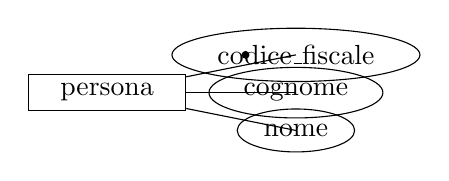
\begin{tikzpicture}[scale=0.8]
\node[rectangle, draw, minimum width=2cm] (persona) at (0,0) {persona};
\node[ellipse, draw] at (3,0.6) {codice\_fiscale};
\node[ellipse, draw] at (3,0) {cognome};
\node[ellipse, draw] at (3,-0.6) {nome};

\draw (persona) -- (3,0.6);
\draw (persona) -- (3,0);
\draw (persona) -- (3,-0.6);

\node[fill=black, circle, scale=0.3] at (2.2,0.6) {};
\end{tikzpicture}
\end{center}

\vspace{0.3cm}

\begin{block}{Schema Relazionale}
\texttt{persona (codice\_fiscale(pk), cognome, nome)}
\end{block}
\end{frame}

% Slide 29
\begin{frame}{Attributi Calcolati}
In caso di presenza di \textbf{attributi calcolati} va aggiunto un vincolo di integrità che specifica il metodo di calcolo.

\vspace{0.5cm}

\begin{example}
Un caso frequente è l'attributo \texttt{età}: questo viene calcolato come differenza di due date (data odierna e data di nascita), e se manca il valore di una di esse il suo valore deve essere \texttt{NULL}.
\end{example}
\end{frame}

\section{Traduzione delle Relazioni}

% Slide 30
\begin{frame}{Trasformazione delle Relazioni}
Si effettua la traduzione delle relazioni, in base a:
\begin{itemize}
\item Numero di entità partecipanti
\item Loro cardinalità
\end{itemize}

\vspace{0.5cm}

Tipologie:
\begin{enumerate}
\item Relazioni uno-a-uno (1,1)
\item Relazioni uno-a-molti (1,N)
\item Relazioni molti-a-molti (N,N)
\item Relazioni ternarie
\end{enumerate}
\end{frame}

% Slide 31
\begin{frame}{Relazioni Uno-a-Uno (1,1)}
Due entità legate da una relazione (1,1) possono essere \textcolor{orange}{\textbf{ridotte a un'unica entità}} che contiene gli attributi sia della prima sia della seconda entità.

\vspace{0.3cm}

\begin{center}
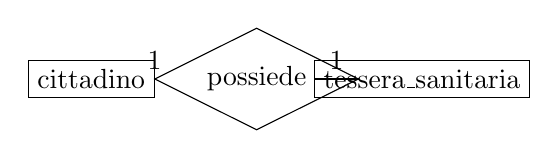
\begin{tikzpicture}[scale=0.7]
\node[rectangle, draw] (citt) at (0,0) {cittadino};
\node[diamond, draw, aspect=2] (poss) at (3,0) {possiede};
\node[rectangle, draw] (tess) at (6,0) {tessera\_sanitaria};

\draw (citt) -- node[above] {1} (poss);
\draw (poss) -- node[above] {1} (tess);
\end{tikzpicture}
\end{center}

\vspace{0.3cm}

La relazione è del tipo 1,1, in quanto un cittadino può possedere una sola tessera sanitaria e ogni tessera sanitaria è unica per ogni cittadino: quindi la relazione è eliminabile e otteniamo un'unica entità con tutti gli attributi.
\end{frame}

% Slide 32
\begin{frame}{Relazioni Uno-a-Uno: Risultato}
\begin{center}
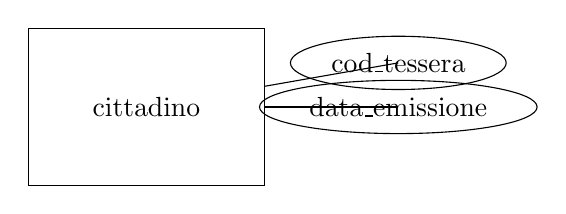
\begin{tikzpicture}[scale=0.8]
\node[rectangle, draw, minimum width=3cm, minimum height=2cm] (citt) at (0,0) {cittadino};
\node[ellipse, draw] at (4,0.7) {cod\_tessera};
\node[ellipse, draw] at (4,0) {data\_emissione};

\draw (citt) -- (4,0.7);
\draw (citt) -- (4,0);
\end{tikzpicture}
\end{center}

Gli attributi della tessera sanitaria vengono incorporati nell'entità cittadino.
\end{frame}

% Slide 33
\begin{frame}{Relazioni Uno-a-Molti (1,N)}
Ogni associazione \textbf{uno a molti} può essere tradotta inserendo un \textcolor{orange}{\textbf{attributo aggiuntivo}} sulla entità da cui la cardinalità massima è 1.

\vspace{0.5cm}

Tale attributo conterrà la \textit{chiave dell'oggetto associato} all'oggetto corrente. Si introduce così una \textcolor{darkblue}{\textbf{chiave esterna (foreign key)}} e, con essa, un vincolo di integrità referenziale.
\end{frame}

% Slide 34
\begin{frame}{Relazioni 1-N: Esempio}
\begin{center}
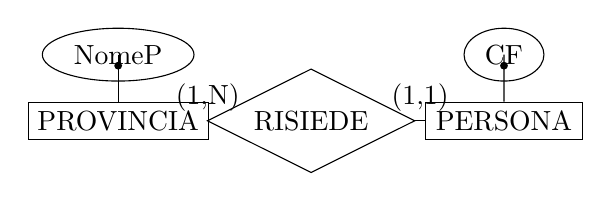
\begin{tikzpicture}[scale=0.7]
\node[rectangle, draw, minimum width=2cm] (prov) at (0,0) {PROVINCIA};
\node[diamond, draw, aspect=2] (ris) at (3.5,0) {RISIEDE};
\node[rectangle, draw, minimum width=2cm] (pers) at (7,0) {PERSONA};

\draw (prov) -- node[above] {(1,N)} (ris);
\draw (ris) -- node[above] {(1,1)} (pers);

\node[ellipse, draw] at (0,1.2) {NomeP};
\node[ellipse, draw] at (7,1.2) {CF};
\draw (prov) -- (0,1.2);
\draw (pers) -- (7,1.2);
\node[fill=black, circle, scale=0.3] at (0,1) {};
\node[fill=black, circle, scale=0.3] at (7,1) {};
\end{tikzpicture}
\end{center}

\vspace{0.3cm}

\begin{block}{Schema Relazionale}
\small
\texttt{PROVINCIA(NomeP, Persona)} \\
\texttt{PERSONA(CF, Nome, NomeP, Dal)} \\
\texttt{FK: NomeP REFERENZIA PROVINCIA}
\end{block}
\end{frame}

% Slide 35
\begin{frame}{Relazioni Molti-a-Molti (N,N)}
Le relazioni \textbf{N,N} non possono essere rappresentate nel modello logico relazionale.

\vspace{0.5cm}

Devono essere tradotte aggiungendo un'\textcolor{orange}{\textbf{entità associativa}} (anche detta entità "ponte") che va messa in relazione con le due entità originali.
\end{frame}

% Slide 36
\begin{frame}{Relazioni N-N: Traduzione}
Una relazione molti a molti che lega due entità si traduce in:
\begin{itemize}
\item Una \textbf{tabella per ogni entità} contenente gli attributi dell'entità
\item Una \textbf{tabella per la relazione} contenente:
\begin{itemize}
\item Gli attributi identificatori delle entità che collega
\item Gli attributi propri
\end{itemize}
\item Gli attributi identificatori della tabella collegata alla relazione compongono la \textcolor{darkblue}{\textbf{chiave esterna}}
\end{itemize}
\end{frame}

% Slide 37
\begin{frame}{Relazioni N-N: Esempio Studente-Corso}
\begin{center}
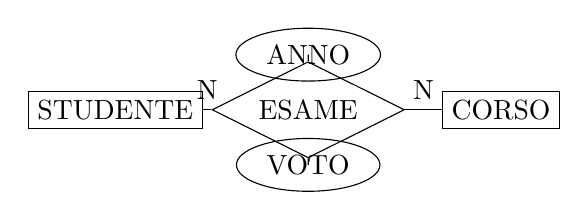
\begin{tikzpicture}[scale=0.7]
\node[rectangle, draw] (stud) at (0,0) {STUDENTE};
\node[diamond, draw, aspect=2] (esame) at (3.5,0) {ESAME};
\node[rectangle, draw] (corso) at (7,0) {CORSO};

\draw (stud) -- node[above] {N} (esame);
\draw (esame) -- node[above] {N} (corso);

\node[ellipse, draw] at (3.5,1) {ANNO};
\node[ellipse, draw] at (3.5,-1) {VOTO};
\draw (esame) -- (3.5,1);
\draw (esame) -- (3.5,-1);
\end{tikzpicture}
\end{center}

\vspace{0.3cm}

\begin{block}{Schema Relazionale}
\small
\texttt{Studente(Matricola, Nome)} \\
\texttt{Corso(Codice, Denominazione)} \\
\texttt{Esame(Matricola, Codice, Anno, Voto)} \\
\texttt{FK: Matricola REFERENZIA Studente} \\
\texttt{FK: Codice REFERENZIA Corso}
\end{block}
\end{frame}

% Slide 38
\begin{frame}{Relazioni N-N: Esempio Impiegato-Progetto}
\begin{center}
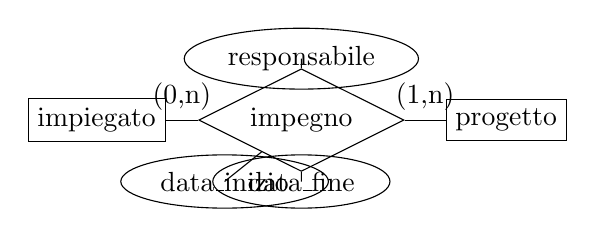
\begin{tikzpicture}[scale=0.65]
\node[rectangle, draw] (imp) at (0,0) {impiegato};
\node[diamond, draw, aspect=2] (impegno) at (4,0) {impegno};
\node[rectangle, draw] (prog) at (8,0) {progetto};

\draw (imp) -- node[above] {(0,n)} (impegno);
\draw (impegno) -- node[above] {(1,n)} (prog);

\node[ellipse, draw] at (4,1.2) {responsabile};
\node[ellipse, draw] at (4,-1.2) {data\_fine};
\node[ellipse, draw] at (2.5,-1.2) {data\_inizio};
\draw (impegno) -- (4,1.2);
\draw (impegno) -- (4,-1.2);
\draw (impegno) -- (2.5,-1.2);
\end{tikzpicture}
\end{center}

Gli attributi della relazione vengono inseriti nella tabella associativa.

\vspace{0.3cm}

\begin{block}{Schema Relazionale}
\footnotesize
\texttt{impiegato (ID\_impiegato(pk), cognome, nome)} \\
\texttt{progetto (ID\_progetto(pk), descrizione)} \\
\texttt{impegno (ID\_impiegato(pk), ID\_progetto(pk), data\_inizio, responsabile)}
\end{block}
\end{frame}

\section{Relazioni Ternarie}

% Slide 39
\begin{frame}{Relazioni Ternarie}
Una \textbf{relazione ternaria} collega logicamente tre entità.

\vspace{0.3cm}

\begin{center}
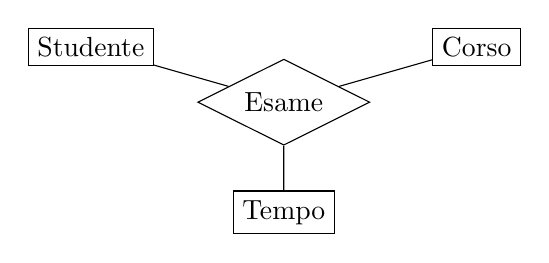
\begin{tikzpicture}[scale=0.7]
\node[rectangle, draw] (stud) at (0,2) {Studente};
\node[diamond, draw, aspect=2] (esame) at (3.5,1) {Esame};
\node[rectangle, draw] (corso) at (7,2) {Corso};
\node[rectangle, draw] (tempo) at (3.5,-1) {Tempo};

\draw (stud) -- (esame);
\draw (corso) -- (esame);
\draw (tempo) -- (esame);
\end{tikzpicture}
\end{center}

\vspace{0.3cm}

\begin{example}
Uno studente può ripetere lo stesso esame in tempi diversi.
\end{example}
\end{frame}

% Slide 40
\begin{frame}{Relazioni Ternarie: Caratteristiche}
Le cardinalità minime raramente sono 1 per tutte le entità coinvolte in una relazione ternaria.

\vspace{0.5cm}

Le cardinalità massime di una relazione n-aria sono (praticamente) sempre \textbf{N}.

\vspace{0.5cm}

\begin{alertblock}{Nota importante}
Se la partecipazione di un'entità E ha cardinalità massima 1, è possibile eliminare la relazione n-aria e legare l'entità E con le altre mediante relazioni binarie.
\end{alertblock}
\end{frame}

% Slide 41
\begin{frame}{Relazioni Ternarie: Esempio Fornitura}
\begin{center}
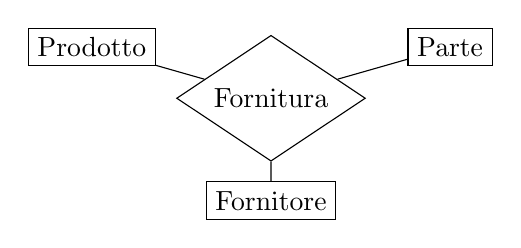
\begin{tikzpicture}[scale=0.65]
\node[rectangle, draw] (dip) at (0,2) {Prodotto};
\node[diamond, draw, aspect=1.5] (forn) at (3.5,1) {Fornitura};
\node[rectangle, draw] (prod) at (7,2) {Parte};
\node[rectangle, draw] (vend) at (3.5,-1) {Fornitore};

\draw (dip) -- (forn);
\draw (prod) -- (forn);
\draw (vend) -- (forn);
\end{tikzpicture}
\end{center}

\begin{itemize}
\item Il venditore A fornisce stampanti al Dipartimento Personale
\item Il venditore B fornisce fotocopiatrici al Dipartimento Ricerca
\end{itemize}
\end{frame}

% Slide 42
\begin{frame}{Relazioni Ternarie: Traduzione}
La relazione ternaria con cardinalità molti a molti viene trasformata nel seguente modo:
\begin{itemize}
\item Ogni \textbf{entità} in una tabella
\item La \textbf{relazione} in una tabella contenente:
\begin{itemize}
\item Tutti gli attributi chiave delle entità collegate
\item L'attributo proprio (se presente)
\end{itemize}
\end{itemize}
\end{frame}

% Slide 43
\begin{frame}{Relazioni Ternarie: Schema Finale}
\begin{block}{Schema Relazionale}
\small
\texttt{Prodotto(CodProd, Nome)} \\
\texttt{Fornitore(CodForn, Telefono)} \\
\texttt{Parte(CodPart, Descrizione)} \\
\texttt{Fornitura(CodPart, CodProd, CodForn, Quantità)} \\
\vspace{0.2cm}
\texttt{FK: CodPart REFERENZIA Parte} \\
\texttt{FK: CodProd REFERENZIA Prodotto} \\
\texttt{FK: CodForn REFERENZIA Fornitore}
\end{block}
\end{frame}

% Slide 44
\begin{frame}{Esempio Complesso: Fattura-Cliente-Prodotto}
\begin{center}
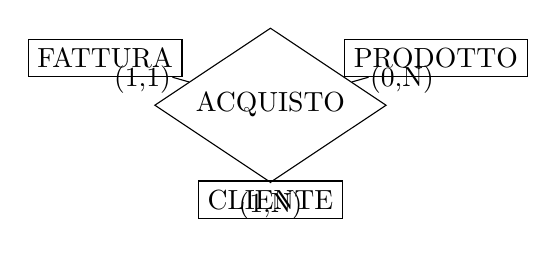
\begin{tikzpicture}[scale=0.6]
\node[rectangle, draw] (fatt) at (0,2) {FATTURA};
\node[diamond, draw, aspect=1.5] (acq) at (3.5,1) {ACQUISTO};
\node[rectangle, draw] (prod) at (7,2) {PRODOTTO};
\node[rectangle, draw] (cli) at (3.5,-1) {CLIENTE};

\draw (fatt) -- node[left] {(1,1)} (acq);
\draw (prod) -- node[right] {(0,N)} (acq);
\draw (cli) -- node[below] {(1,N)} (acq);
\end{tikzpicture}
\end{center}

La relazione ternaria con una cardinalità (1,1) può essere scomposta in relazioni binarie.
\end{frame}

% Slide 45
\begin{frame}{Scomposizione Relazione Ternaria}
\begin{center}
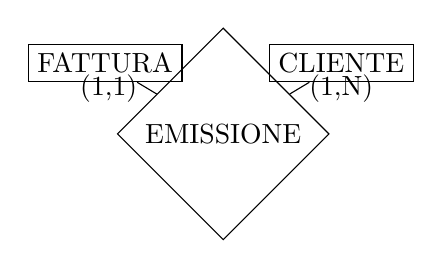
\begin{tikzpicture}[scale=0.6]
\node[rectangle, draw] (fatt) at (0,1.5) {FATTURA};
\node[diamond, draw] (emis) at (2.5,0) {EMISSIONE};
\node[rectangle, draw] (cli) at (5,1.5) {CLIENTE};

\draw (fatt) -- node[left] {(1,1)} (emis);
\draw (emis) -- node[right] {(1,N)} (cli);
\end{tikzpicture}
\end{center}
\end{frame}

\section{Relazioni Ridondanti}

% Slide 46
\begin{frame}{Eliminare le Relazioni Ridondanti}
Una \textbf{relazione ridondante} è una relazione definita tra due entità e che è equivalente nel significato a un'altra relazione tra le stesse due entità che passa attraverso un'entità intermedia.

\vspace{0.5cm}

\begin{example}
\begin{itemize}
\item Una persona abita in una provincia
\item Una persona risiede in un paese
\item Il paese si trova in una provincia
\end{itemize}
\end{example}

La prima relazione è \textcolor{red}{ridondante} rispetto alle altre due.
\end{frame}

% Slide 47
\begin{frame}{Ridondanza: Esempio Visivo}
\begin{center}
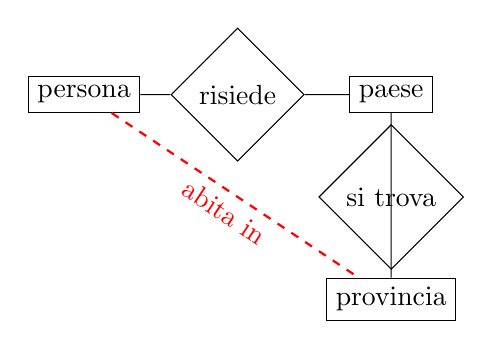
\begin{tikzpicture}[scale=0.65]
\node[rectangle, draw] (pers) at (0,2) {persona};
\node[diamond, draw] (ris) at (3,2) {risiede};
\node[rectangle, draw] (paese) at (6,2) {paese};
\node[diamond, draw] at (6,0) {si trova};
\node[rectangle, draw] (prov) at (6,-2) {provincia};

\draw (pers) -- (ris);
\draw (ris) -- (paese);
\draw (paese) -- (6,0);
\draw (6,0) -- (prov);

% Relazione ridondante
\draw[red, dashed, thick] (pers) -- node[below, sloped] {abita in} (prov);
\end{tikzpicture}
\end{center}

La relazione tratteggiata è \textcolor{red}{eliminabile}.
\end{frame}

% Slide 48
\begin{frame}{Definizione delle Chiavi}
Aggiungere anche la definizione delle chiavi:
\begin{itemize}
\item Le \textbf{chiavi artificiali} iniziano con \texttt{ID}
\item Per convenzione usiamo \texttt{ID} \textit{maiuscolo} per la chiave primaria
\item Indichiamo con \texttt{id} \textit{minuscolo} le chiavi esterne
\end{itemize}

\vspace{0.5cm}

\begin{example}
\texttt{STUDENTE(ID\_studente(PK), nome, cognome, id\_classe(FK))} \\
\texttt{CLASSE(ID\_classe(PK), sezione, anno)}
\end{example}
\end{frame}

% Slide 49
\begin{frame}{Vincoli da Considerare}
\begin{enumerate}
\item Vincoli \textbf{NOT NULL} per gli attributi obbligatori
\item Vincoli di \textbf{interdipendenza} di valori nulli
\item Vincoli di \textbf{chiave} (primarie e non)
\item Vincoli di \textbf{foreign key} che provengono dalla traduzione di relazioni
\item Vincoli di \textbf{generalizzazione}, formulati come vincoli insiemistici
\end{enumerate}
\end{frame}

% Slide 50
\begin{frame}{Vincoli di Cardinalità}
\begin{block}{Partecipazione obbligatoria (cardinalità minima 1)}
Diventa vincolo di inclusione o foreign key dalla relazione che corrisponde all'entità verso quella che corrisponde alla ER-relazione
\end{block}

\vspace{0.3cm}

\begin{block}{Funzionalità (cardinalità massima 1)}
Diventa vincolo di chiave sulla relazione che corrisponde alla ER-relazione
\end{block}
\end{frame}

% Final slide
\begin{frame}[plain]
\begin{center}
\Huge \textcolor{darkblue}{Grazie per l'attenzione!}
\vspace{2cm}

\Large Domande?
\end{center}
\end{frame}

\end{document}
